\begin{document}
To start off with the clusters profiling, we have performed the Pearson's chi-squared test for all categorical and binary variables of our dataset. This way we can know whether our clusters are well established and how dependant is each one of these variables to their actual cluster.

So, after running the test, we have seen a generally low p-value among almost all of these variables. That means we cannot discard our null hypothesis which is that the variables are not dependant on the cluster.

Chi squared test results are shown in the table below.
\newline


\begin{table}[h!]
\centering
\begin{tabular}{|c| c| c|}
 \hline
 \textbf{Variable} & \textbf{X-squared} & \textbf{p-value}\\ [0.5ex]
 \hline\hline
 gender & 8.9301 & 0.0115\\
 match & 159.6 & 2.2e-16\\
 samerace & 85.201 & 2.2e-16\\
 race\_o & 15.997 & 0.04242\\
 dec\_o & 501.3 & 2.2e-16\\
 field\_cd & 812.14 & 2.2e-16\\
 race & 376 & 2.2e-16\\
 goal & 334.47 & 2.2e-16\\
 date & 440.09 & 2.2e-16\\
 go\_out & 517.58 & 2.2e-16\\
 dec & 501.3 & 2.2e-16\\
 university & 3519.5 & 2.2e-16\\
 \hline
\end{tabular}
\caption{Chi-squared and p-value for categorical and boolean variables}
\label{table:1}
\end{table}

\newpage
On the other hand, for numerical variables we have done a simple mean operation for each of the different clusters.

The results of the arithmetic mean for each variable and cluster are shown in the table below.
\newline

\begin{table}[h!]
\centering
\begin{tabular}{|c| c| c| c|}
 \hline
 
 \textbf{Variable} & \textbf{Cluster 1} & \textbf{Cluster 2} & \textbf{Cluster 3}\\ [0.5ex]
 \hline\hline
 round & 16.04312 & 17.31410 & 17.67141\\
 order & 8.506250 & 8.985161 & 9.416370\\
 int\_corr & 0.1560750 & 0.2065128 & 0.2514472\\
 age\_o & 25.67563 & 26.19456 & 26.76750 \\
 pf\_o\_att & 22.98625  & 24.20610 & 24.41044\\
 pf\_o\_sin & 16.92063 & 17.65622 & 17.86714\\
 pf\_o\_int & 22.12750 & 20.58203 & 20.38078\\
 pf\_o\_fun & 17.17000 & 17.34378 & 16.9822\\
 pf\_o\_amb & 9.688125 & 9.356966 & 9.288256\\
 pf\_o\_sha & 11.09437 & 10.87881 & 11.09964\\
 attr\_o & 15.38500 & 15.44847 & 16.13642\\
 sinc\_o & 18.40125 & 18.29349 & 18.11862\\
 intel\_o & 19.01250 & 19.25639 & 18.66311\\
 fun\_o & 16.14313 & 15.90437 & 16.09371\\
 amb\_o & 17.61375 & 17.70816 & 17.30486\\
 shar\_o & 13.67812 & 13.61006 & 13.95492\\
 age & 25.68500 & 26.26793 & 26.62040\\
 mn\_sat & 2.3375 & 1284.8013 & 1301.1198\\
 tuition & 36.97812 & 21812.44683 & 22251.20641\\
 imprace & 3.715625 & 3.034625 & 4.148280\\
 income & 41197.10 & 47766.52 & 52105.42\\
 like & 6.205938 & 6.427040 & 5.580071\\
 imprelig & 3.905000 & 3.574608 & 3.945433\\
 diff\_age & 3.595625 & 3.281946 & 4.033215\\
 \hline
\end{tabular}
\caption{Average values for each numerical variable and cluster}
\label{table:1}
\end{table}


We have also checked the match rate for each of the clusters, results of which are shown in the table below.

\begin{table}[h!]
\centering
\begin{tabular}{|c| c|} 
 \hline
 \textbf{Cluster} & \textbf{\% of match} \\ [0.5ex]
 \hline\hline
 1 & 17.312500\\
 2 & 25.886232\\
 3 & 4.507711\\
 \hline
\end{tabular}
\caption{Percentage of match for each cluster}
\label{table:1}
\end{table}

\newpage
After these tables, we can see some of the differences between the three clusters. We are going to outline them, but the reader should take into account that, as stated before, the p-values are low and therefore we cannot affirm that these differences are significant enough, so take the following results with care. The first difference, as shown in table 6, is the rate of match. While the third cluster presents the lowest match rate with roughly 4.5 percent, over 1 out of 4 meetings put classified in the second one end in being a match.

Another noticeable difference we find is about cluster 1. This one includes those meetings which the main subject has the least grade on the exam to enter college (mn\_sat) as well as the sum of money charged to enter college (tuition).

Moreover, we can see by joining tables 5 and 6 that subjects who care less about his/her date generally end up having a higher match rate, as we could have guessed. This could specially importamt in a country so much ethnic-diverse as United States is.

Same thing happens age difference between two dating mates (diff\_ages), where we can see an inversely proportional relation between age difference and match chance.
\newline
\newline

Our next step in profiling is the study of the clusters and variables using plots and charts.
\newline
First of all, we grouped the data into two groups: those observations who ended up in a match and those which did not. We also divided them into categorical/binary and numerical. We can see the results in the following six figures.

\begin{figure}
  \centering
  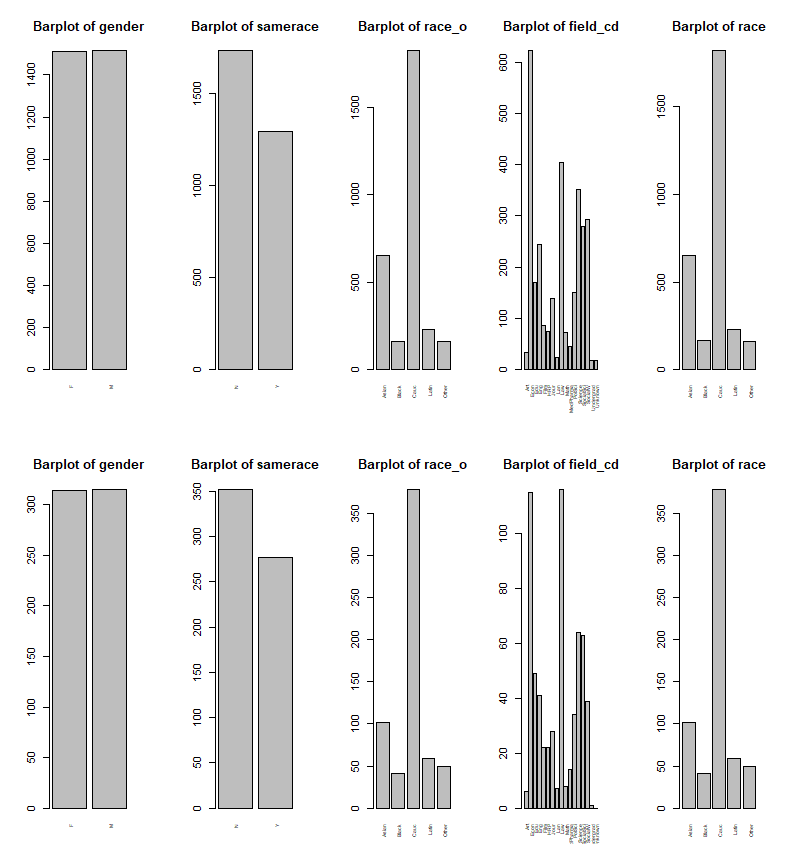
\includegraphics[width= 16cm, height=17cm]{images/profiling/CPG_match_gender_race.png}
  \caption{Study of categorical and binary variables depending on variable match. Above, if it is not match; below if it is a match.}
  \label{fig:indiv}
\end{figure}

\begin{figure}
  \centering
  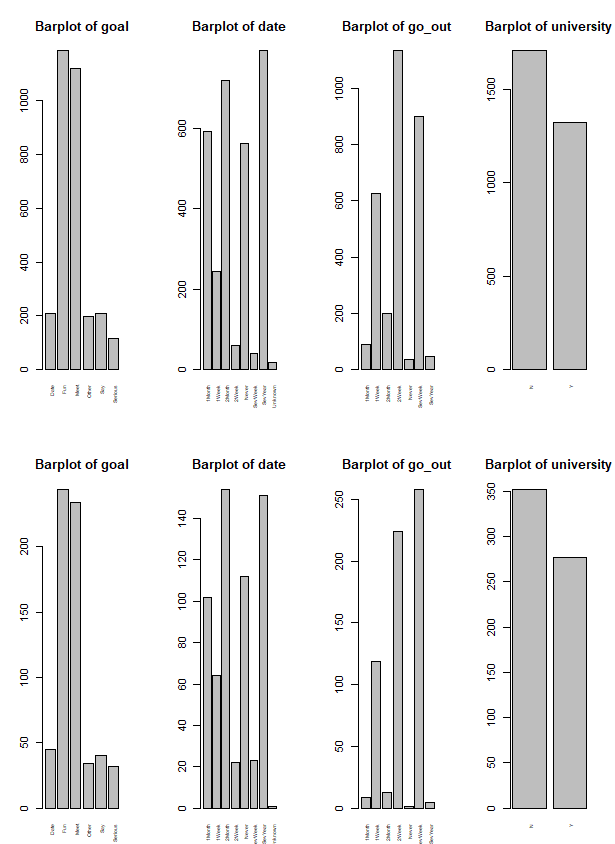
\includegraphics[width= 16cm, height=17cm]{images/profiling/CPG_match_goal_university.png}
  \caption{Study of categorical and binary variables depending on variable match. Above, if it is not match; below if it is a match.}
  \label{fig:indiv}
\end{figure}

\begin{figure}
  \centering
  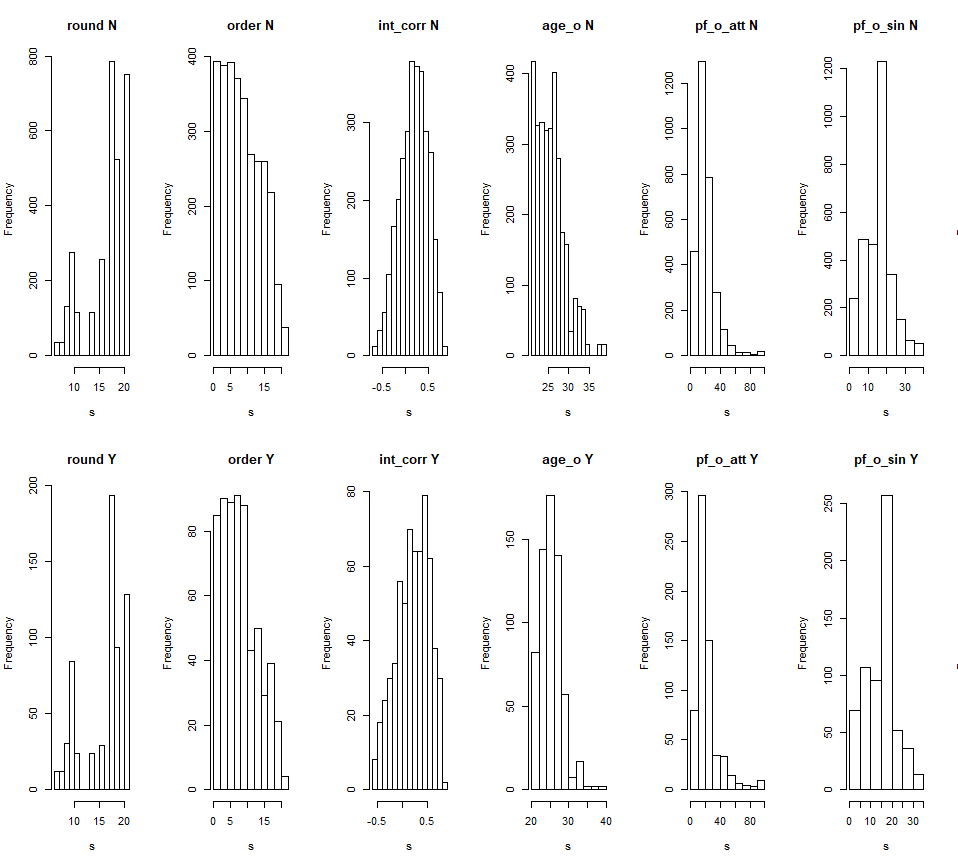
\includegraphics[width= 16cm, height=14cm]{images/profiling/CPG_match_numerical_round_pfosin.png}
  \caption{Study of numerical variables depending on variable match. Above, if it is not match; below if it is a match.}
  \label{fig:indiv}
\end{figure}

\begin{figure}
  \centering
  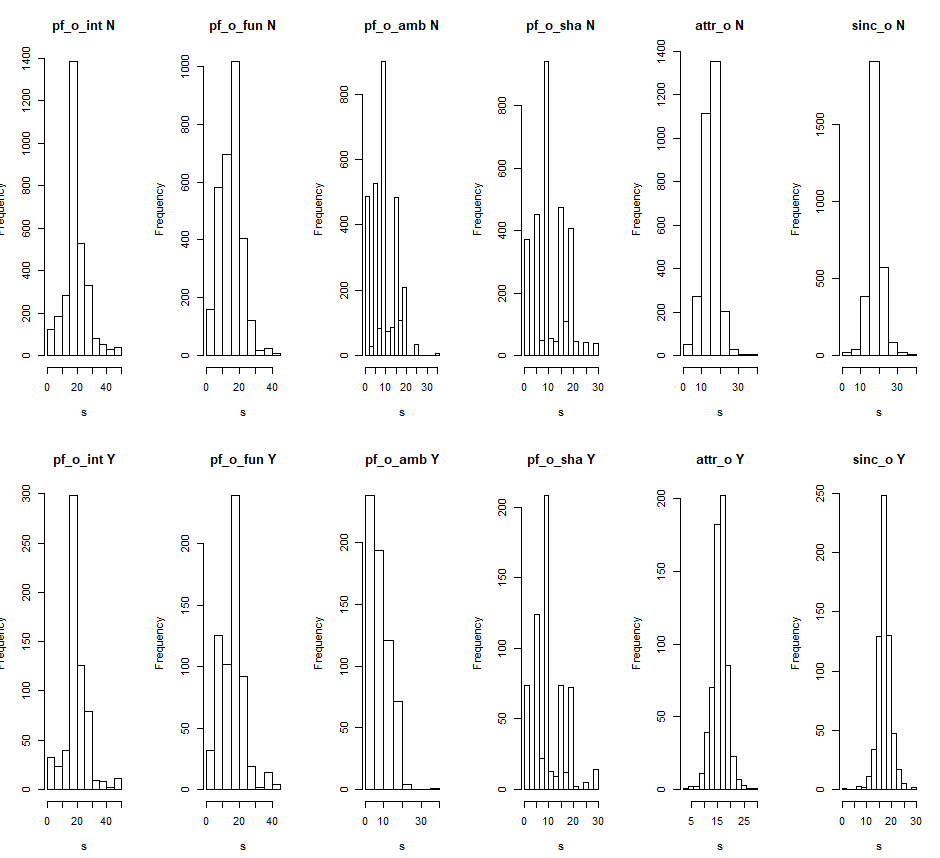
\includegraphics[width= 16cm, height=14cm]{images/profiling/CPG_match_numerical_pfoint_sinco.png}
  \caption{Study of numerical variables depending on variable match. Above, if it is not match; below if it is a match.}
  \label{fig:indiv}
\end{figure}

\begin{figure}
  \centering
  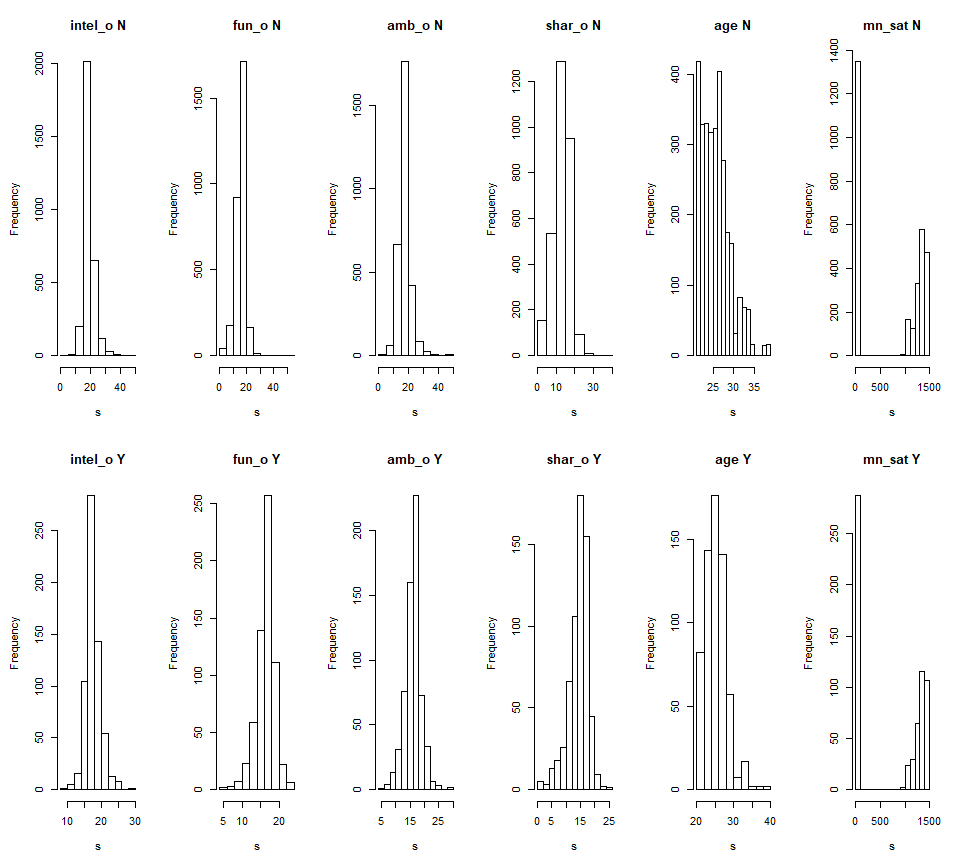
\includegraphics[width= 16cm, height=14cm]{images/profiling/CPG_match_numerical_intelo_mnsat.png}
  \caption{Study of numerical variables depending on variable match. Above, if it is not match; below if it is a match.}
  \label{fig:indiv}
\end{figure}

\begin{figure}
  \centering
  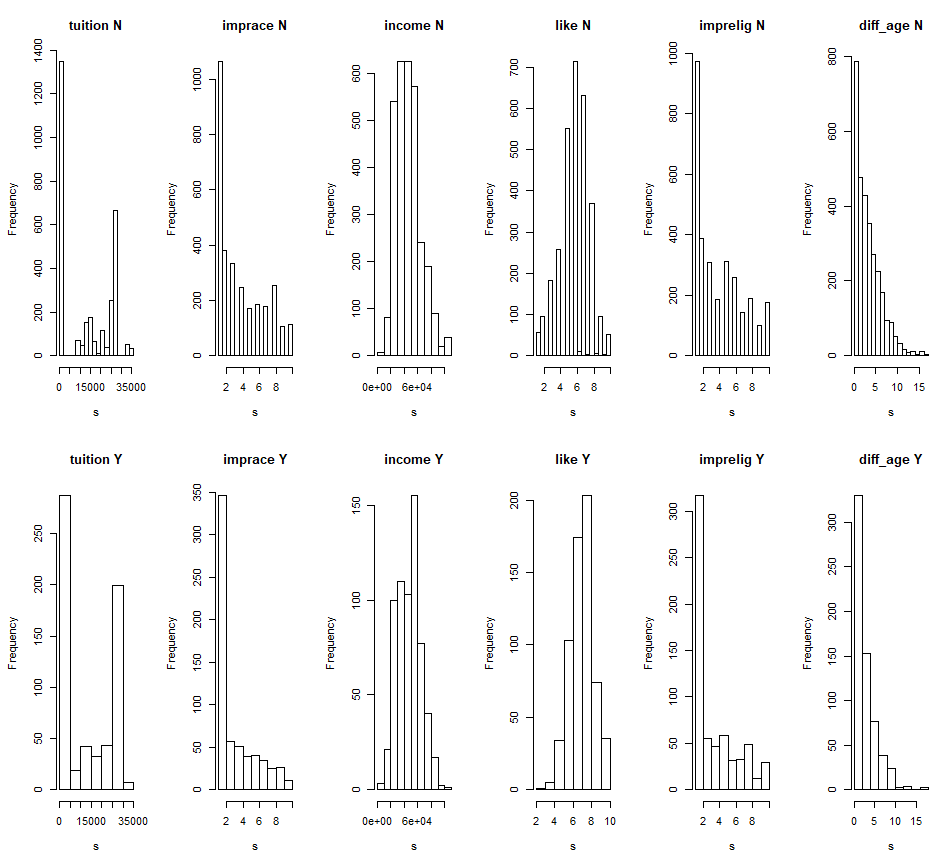
\includegraphics[width= 16cm, height=14cm]{images/profiling/CPG_match_numerical_tuition_diffage.png}
  \caption{Study of numerical variables depending on variable match. Above, if it is not match; below if it is a match.}
  \label{fig:indiv}
\end{figure}

\newpage
We are going to describe and analyze the resulting plots. Again, the reader should take into account that the p-values are low, so the following points might not be significant enough.

We can see in figure 34 that some of the important properties that most influence in whether a date ends up in a match or not are the importance of the religion, the importance of the race and difference of age.

For the importance of the religion, we can observe that the difference in the amount of subjects that do not mind about this at all and the amount of people that mind is larger when a date ends up in a match than on the other way.

It occurs the same way for the importance of the race, favouring those subjects who do not mind at all about his or her partner's race or ethnic group.

For the difference of age, we can observe that a match-ending date has higher chance to happen when the two subjects have a very low or null difference of age.

Income also has a positive direct relation towards a date ending in a match. It seems that subjects who end up matching have a slight higher income.

In figure 30 we can see a very subtle fact. This is that people who go out several times a week (this is the variable which reflects going out most times a week) tend to be more positive towards having a match.

Quite in a similar way it occurs to variable date. Those subjects who go out several times a week (maximum value for the variable) have a higher chance to end the date up in a match.

Regarding to field of study, we see a clear enhancement for the law field. While the other fields remain quite equal from a plot to the other, law field increases the most by far.

We do not see any evidence of whether being the same race affects towards the date ending up in a match or not. Although, we can see a subtle change in the race plot, where Asian subjects are more likely (not by much although) to not ending the date as a match.

Also, those who prefer an ambitious partner (figure 32) seem to have less chances to have a match. As we can observe, while most of subjects who do not end with a match have a more or less high preference about this, those who finally match at the end of the date present a lower rate of preference of ambition.
\newline\newline


We have also grouped the data in three groups depending on which cluster is each observation fit in, as we can see in the next eight figures. Note that, just like we did before, we have divided them on whether they are categorical/binary variables or numerical.

\begin{figure}
  \centering
  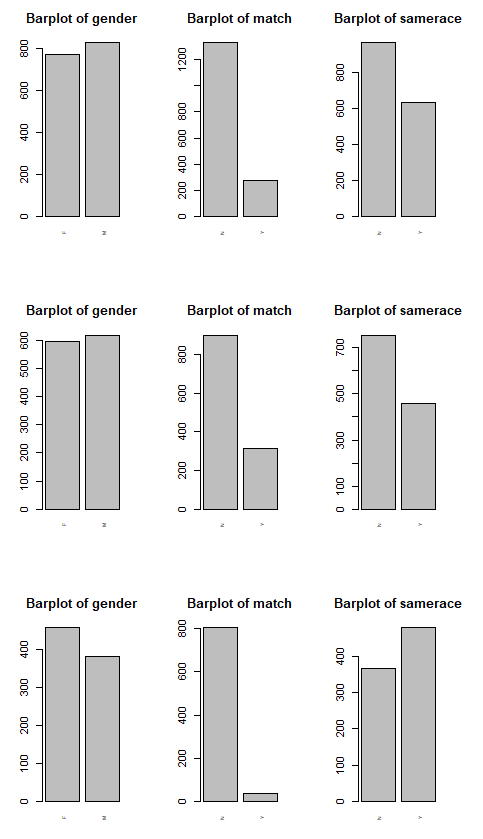
\includegraphics[width= 11cm, height=19cm]{images/profiling/CPG_cluster_gender_samerace.png}
  \caption{Study of categorical and binary variables depending on the cluster they are fit in. From top to bottom, clusters 1, 2 and 3.}
  \label{fig:indiv}
\end{figure}

\begin{figure}
  \centering
  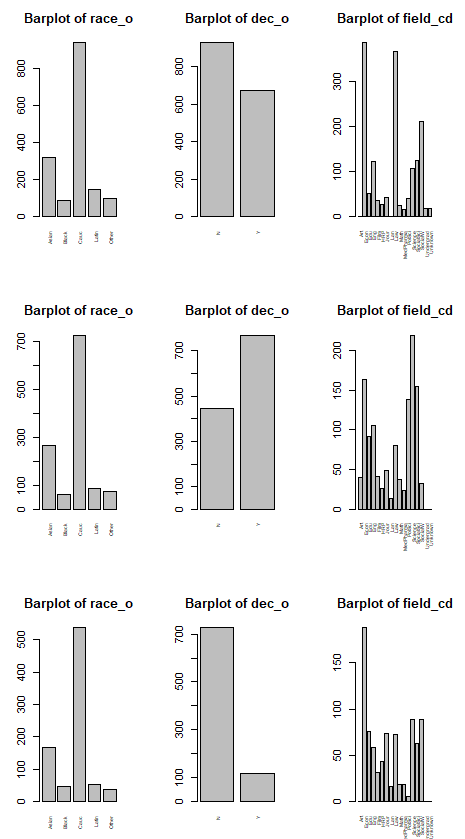
\includegraphics[width= 11cm, height=19cm]{images/profiling/CPG_cluster_raceo_fieldc.png}
  \caption{Study of categorical and binary variables depending on the cluster they are fit in. From top to bottom, clusters 1, 2 and 3.}
  \label{fig:indiv}
\end{figure}

\begin{figure}
  \centering
  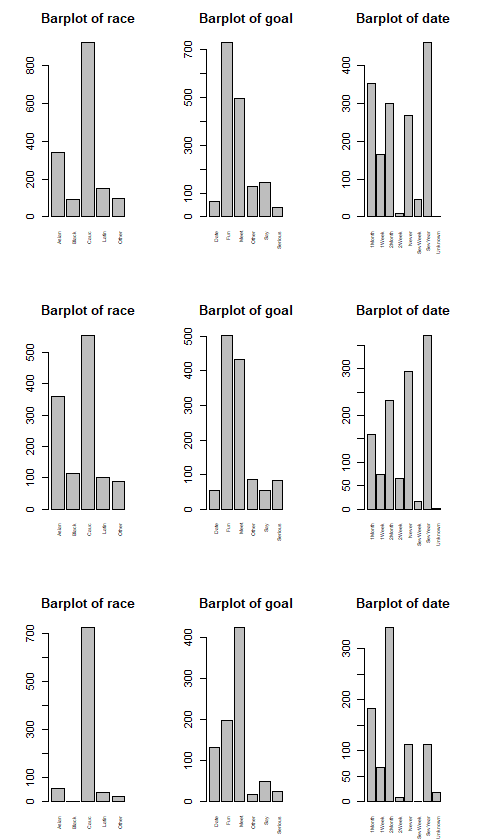
\includegraphics[width= 11cm, height=19cm]{images/profiling/CPG_cluster_race_date.png}
  \caption{Study of categorical and binary variables depending on the cluster they are fit in. From top to bottom, clusters 1, 2 and 3.}
  \label{fig:indiv}
\end{figure}

\begin{figure}
  \centering
  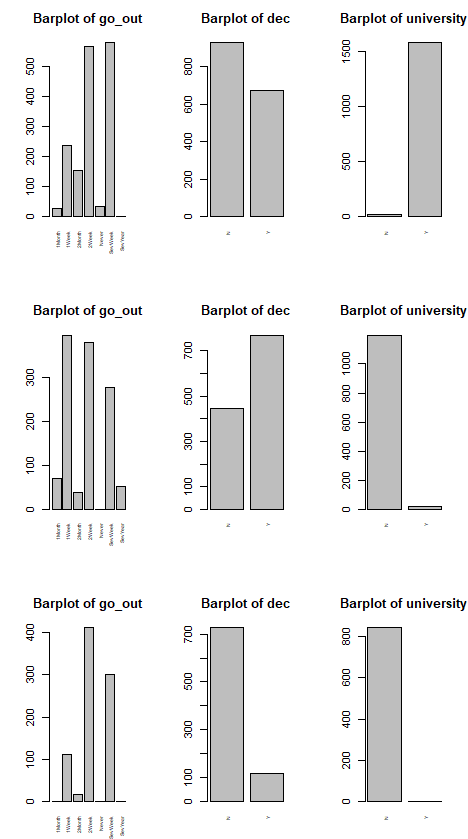
\includegraphics[width= 11cm, height=19cm]{images/profiling/CPG_cluster_goout_university.png}
  \caption{Study of categorical and binary variables depending on the cluster they are fit in. From top to bottom, clusters 1, 2 and 3.}
  \label{fig:indiv}
\end{figure}

\begin{figure}
  \centering
  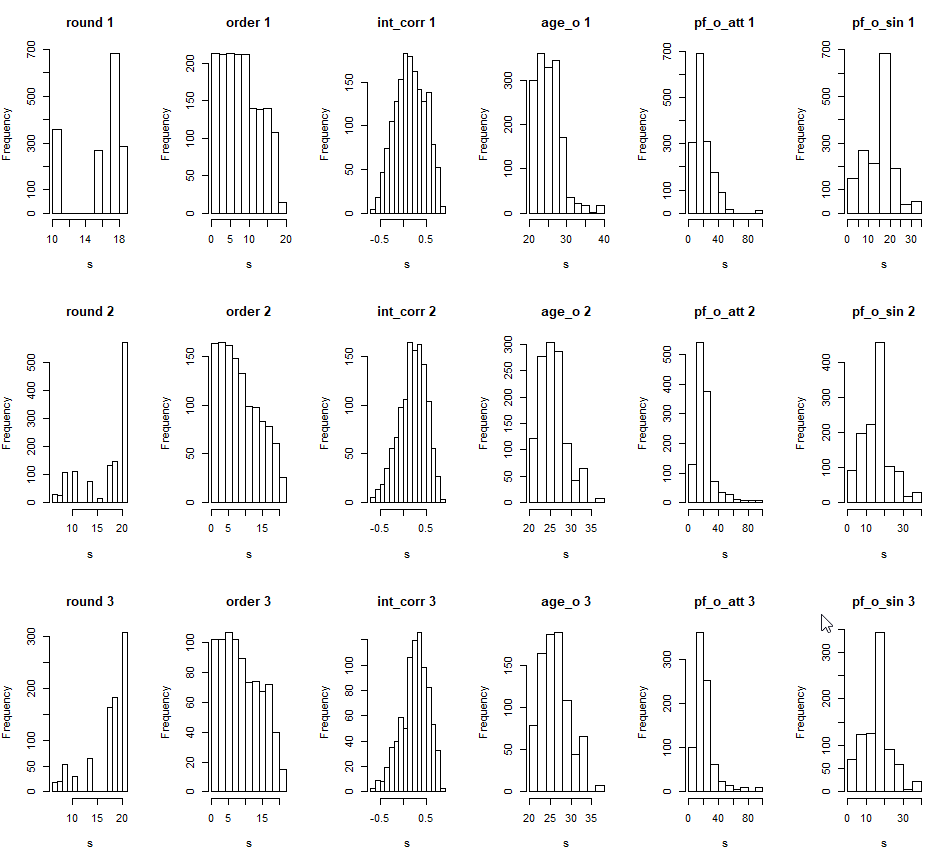
\includegraphics[width= 16cm, height=14cm]{images/profiling/CPG_cluster_numerical_round_pfosin.png}
  \caption{Study of numerical variables depending on the cluster they are fit in. From top to bottom, clusters 1, 2 and 3.}
  \label{fig:indiv}
\end{figure}

\begin{figure}
  \centering
  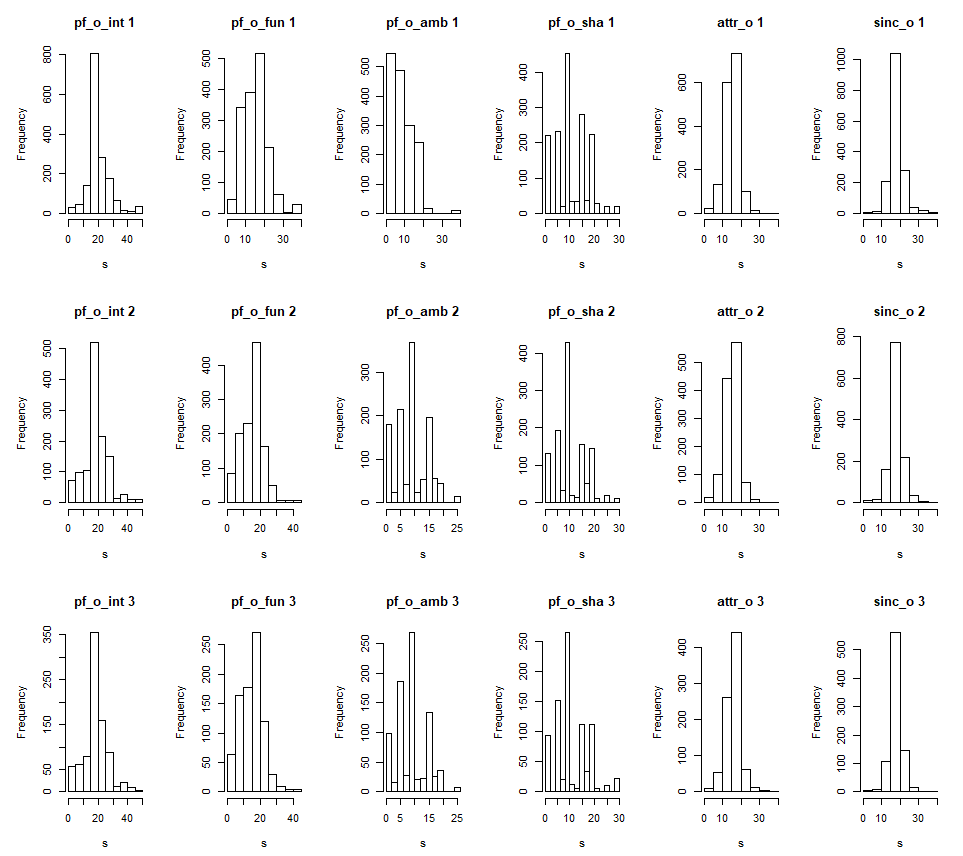
\includegraphics[width= 16cm, height=14cm]{images/profiling/CPG_cluster_numerical_pfoint_sinco.png}
  \caption{Study of numerical variables depending on the cluster they are fit in. From top to bottom, clusters 1, 2 and 3.}
  \label{fig:indiv}
\end{figure}

\begin{figure}
  \centering
  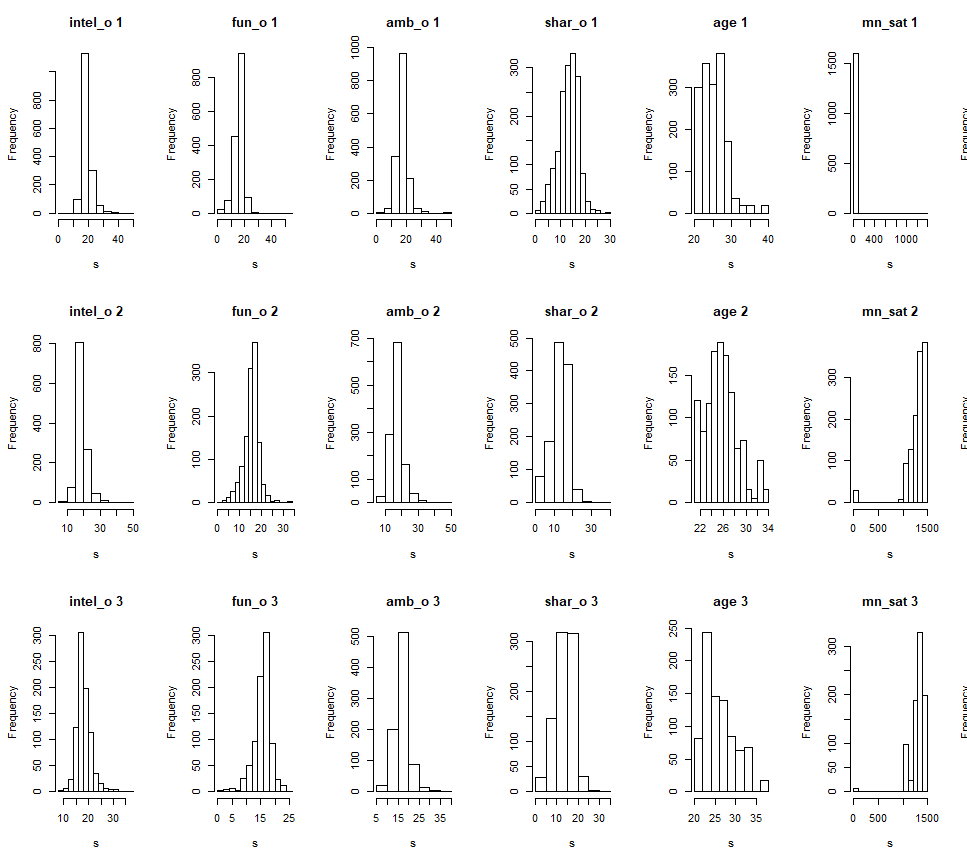
\includegraphics[width= 16cm, height=14cm]{images/profiling/CPG_cluster_numerical_intelo_mnsat.png}
  \caption{Study of numerical variables depending on the cluster they are fit in. From top to bottom, clusters 1, 2 and 3.}
  \label{fig:indiv}
\end{figure}

\begin{figure}
  \centering
  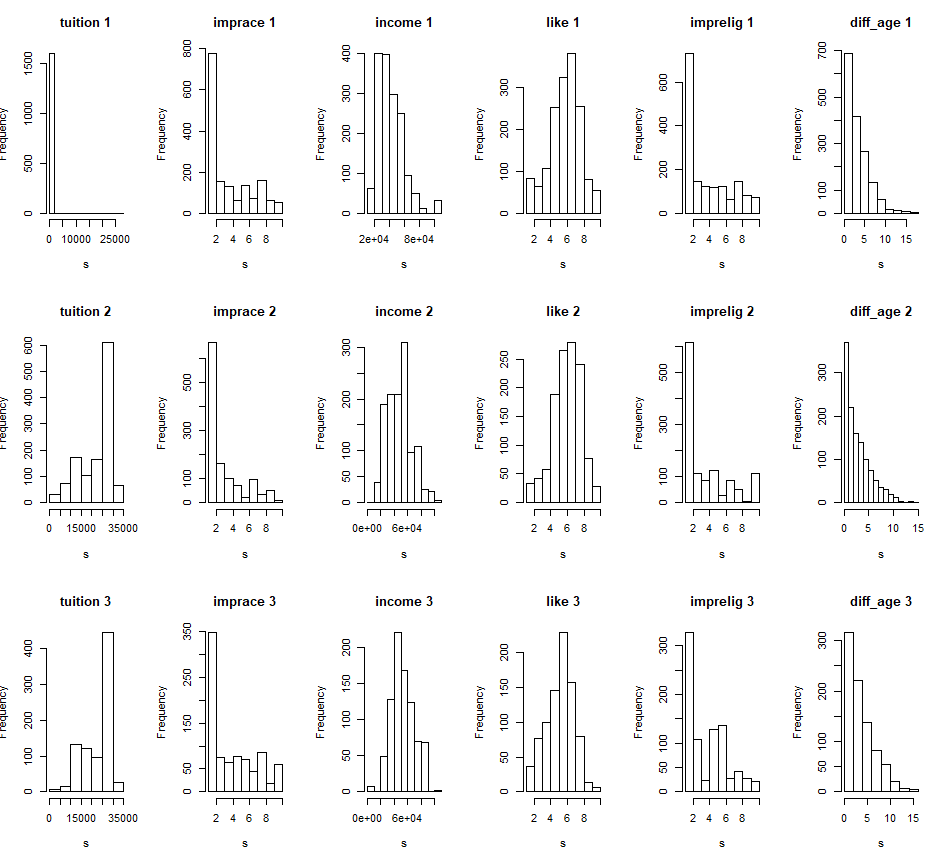
\includegraphics[width= 16cm, height=14cm]{images/profiling/CPG_cluster_numerical_tuition_diffage.png}
  \caption{Study of numerical variables depending on the cluster they are fit in. From top to bottom, clusters 1, 2 and 3.}
  \label{fig:indiv}
\end{figure}

\newpage
First of all, we can see that cluster 3 presents a very low rate of match observations, while first and second clusters have a higher rate, being the second one the one with the highest of all (figure 35).

We can observe that one of the main criteria to separate clusters has been whether the subject has been to University or not (figure 38). As we see in figure 38,  while most subjects that have been to college are placed in cluster 1, the other two clusters mainly have subjects who have not attended University.

Also, we can get to a similar conclusion about importance of religion than we did earlier on. We can observe that cluster 3 is the one that presents a higher rate of subjects who give more importance to the religion of their date (figure 42). If we merged this observation with cluster 3 being the one with the lowest match rate by far, we could see this as a reason.

This last cluster is the one presenting a higher rate of young subjects as well (figure 41).

Moreover, clusters 1 and 2 present a very higher rate of subjects who go frequently on a date compared to cluster 3, whose subjects tend to go on a date in a less frequent manner.
\newline \newline

So, in summary, we could say this is what characterize each cluster:
\begin{itemize}
	\item \textbf{Cluster 1:} This cluster's main characteristic is that most of the subjects that it contains have attended University. This cluster's subjects' field of study concentrate between business/finances and law.
    \item \textbf{Cluster 2:} This cluster is the one with the highest match rate. Together with cluster 3, this cluster presents a very poorly number of subjects who have attended University. Moreover, this cluster's subjects' most frequent field of study is science and most frequent race is asian.
    \item \textbf{Cluster 3:} This cluster has a very poor match rate while presenting the highest rate of all three in subjects whose field of study is business or finances. Cluster 3 also presents the highest rate of Caucasian subjects as well as subjects whose main goal of participating is to meet new poeple. Finally, subjects in this cluster tend to rate religion's importance higher.
\end{itemize}

\end{document}